\begin{figure}[htp]
   \centering
   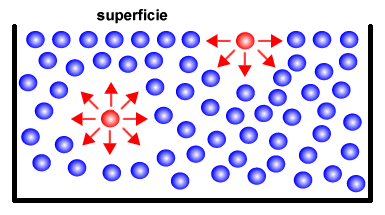
\includegraphics[width=8cm]{immagini/tensione_superficiale.png}
\end{figure}

Consideriamo una generica particella all'interno di un liquido. Essa è sottoposta a varie interazioni in tutte le direzioni, le quali sono omogenee. 
   
Consideriamo ora una particella che sta in superficie (la superficie in gergo tecnico si chiama \textit{pelo libero del liquido}). Su di essa si esercitano varie interazioni dovute alla particelle circostanti nella parte interna del liquido, ma ne vengono a mancare altre, quindi l'entità di interazione su questa particella non sarà la stessa di quella interna.

Se le interazioni che sente la particella sono attrattive, ne viene fuori che in superficie tende ad assumere la forma di una goccia. Dunque queste interazioni sono responsabili della forma delle superfici dei liquidi.

Con tensione superficiale si individua un lavoro, che è il lavoro necessario per aumentare la superficie di un liquido e si può misurare in $N/m$ oppure in $erg/m^2(=0.001N/m)$. Se usiamo quest'ultima unità di misura, essa rappresenterà il lavoro necessario per aumentare di $1cm^2$  la superficie di un liquido.

Attenzione! La temperatura ha un ruolo determinante nel modificare l'entità delle interazioni, per cui è importante vedere a che temperatura misurare la tensione superficiale.

\hspace{0.5cm}\begin{minipage}{0.35 \textwidth}
   \begin{figure}[H]
       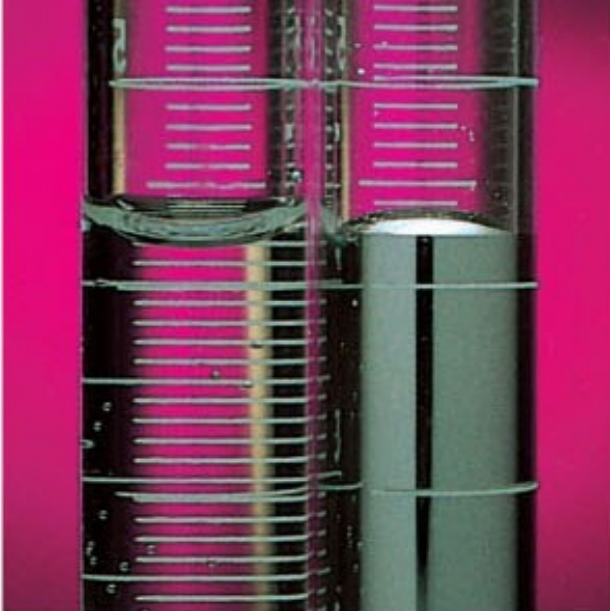
\includegraphics[width=5cm]{immagini/menischi.png}
   \end{figure}
\end{minipage}
\begin{minipage}{0.6 \textwidth}
   \vspace{0.6cm}Abbiamo visto che nei matracci si forma un menisco.
   Questi matracci sono dotati di tacche di 0.1 mL che rappresentano la risoluzione massima. In realtà attraverso le pipette il volume di una tacca può essere diviso in due gocce da 0.05 mL.

   I menischi però hanno una forma concava, quindi come si fa a capire a che volume ci troviamo? In genere si legge il valore del menisco inferiore.

   Va però da notare che a seconda del liquido il menisco ha forma diversa, ad esempio l'acqua ha menisco concavo, il mercurio convesso. Ciò è dovuto alla diversa tensione superficiale.
\end{minipage}

\vspace{0.2cm}Quindi la sfericità delle gocce d'acqua dipende dalle interazioni dei legami ad idrogeno.

A questo punto possiamo separare le superfici in due grandi categorie:

\begin{itemize}
   \item Superfici idrofobiche
   \item Superfici idrofile
\end{itemize}

Una superficie idrofobica è una superficie che si bagna poco, la cui composizione è tale da non dare luogo a consistenti interazioni con le molecole dell'acqua. In questi casi la goccia d'acqua mantiene la sua forma e c'è un contatto minimo con la superficie, che può essere misurato tramite l'angolo di contatto.

In un superficie idrofila invece l'angolo di contatto è di qualche grado.

Quindi le interazioni determinano anche le proprietà che l'acqua mostrerà a contatto con certi materiali.

Inoltre a causa della tensione superficiale è possibile che corpi più densi dell'acqua possano galleggiare.